\chapter{Exploratory NCCL Symmetric-Memory Study}\label{app:nccl-preliminary}

This appendix preserves a later exploratory comparison that is not part of the reconciled main campaign and contributes no evidence to the research-question answers. Its incomplete metadata prevent a device-initiation or application-transfer claim, but the supplied medians identify a candidate for a controlled follow-up.

\section{Protocol and Evidence Boundary}\label{sec:nccl-preliminary-method}

The study compares NCCL~2.18.5 with ordinary allocation, NCCL~2.31.2 with ordinary allocation, and NCCL~2.31.2 with \texttt{ncclMemAlloc} and symmetric window registration on four A100 GPUs. The available summary contains three-run median latencies for 21 allreduce and 19 all-to-all sizes. Comparing versions and comparing the two 2.31.2 configurations answer different questions; the latter still combines allocation and registration.

Symmetric buffers do not establish that user kernels invoked NCCL's device API \cite{nvidia_nccl_registration_2026,nvidia_nccl_device_2026}. Datatype, exact source and launch configuration, completion boundary, warm-up, correctness output, and individual trial timings are unavailable. No uncertainty intervals are reconstructed, and the supplied eight-byte cell is not assumed to be one FP64 sum. The study identifies candidates for follow-up rather than modifying the main campaign's ranking.

\section{Exploratory Results}\label{sec:nccl-preliminary-results}

Table~\ref{tab:m-nccl-preliminary} retains representative gains and regressions from the supplied three-run medians.

\begin{table}[htbp]
\centering
\caption{Preliminary NCCL medians in \,$\mu$s. Plain and symmetric refer to version 2.31.2; the final column divides the 2.18.5 latency by the symmetric latency.}
\label{tab:m-nccl-preliminary}
\footnotesize
\begin{tabular}{llrrrr}
\toprule
Operation & Size & 2.18.5 & Plain & Symmetric & Ratio\\
\midrule
Allreduce & 8\,B & 12.4 & 12.6 & 7.5 & $1.65\times$\\
 & 32\,KiB & 18.4 & 18.5 & 10.6 & $1.74\times$\\
 & 256\,KiB & 19.2 & 19.3 & 22.7 & $0.85\times$\\
 & 1\,MiB & 44.5 & 34.1 & 33.5 & $1.33\times$\\
 & 16\,MiB & 182.0 & 202.1 & 156.4 & $1.16\times$\\
\midrule
All-to-all & 64\,B & 11.1 & 13.8 & 14.0 & $0.79\times$\\
 & 1\,KiB & 11.0 & 12.7 & 12.6 & $0.87\times$\\
 & 8\,MiB & 63.9 & 68.1 & 59.6 & $1.07\times$\\
 & 16\,MiB & 102.2 & 106.1 & 89.2 & $1.15\times$\\
\bottomrule
\end{tabular}
\end{table}

\subsection{Small Allreduce Candidate}

Across the supplied 4\,B--32\,KiB cells, symmetric allocation and registration improve latency by approximately 1.54--1.74 times relative to 2.18.5. At eight bytes the reduction from 12.4 to 7.5\,$\mu$s is approximately 40\% lower latency. Plain 2.31.2 remains at 12.6\,$\mu$s, so the version update alone does not reproduce this small-message gain. The advantage reverses at intermediate sizes, including 256 and 512\,KiB.

\begin{figure}[htbp]
\centering
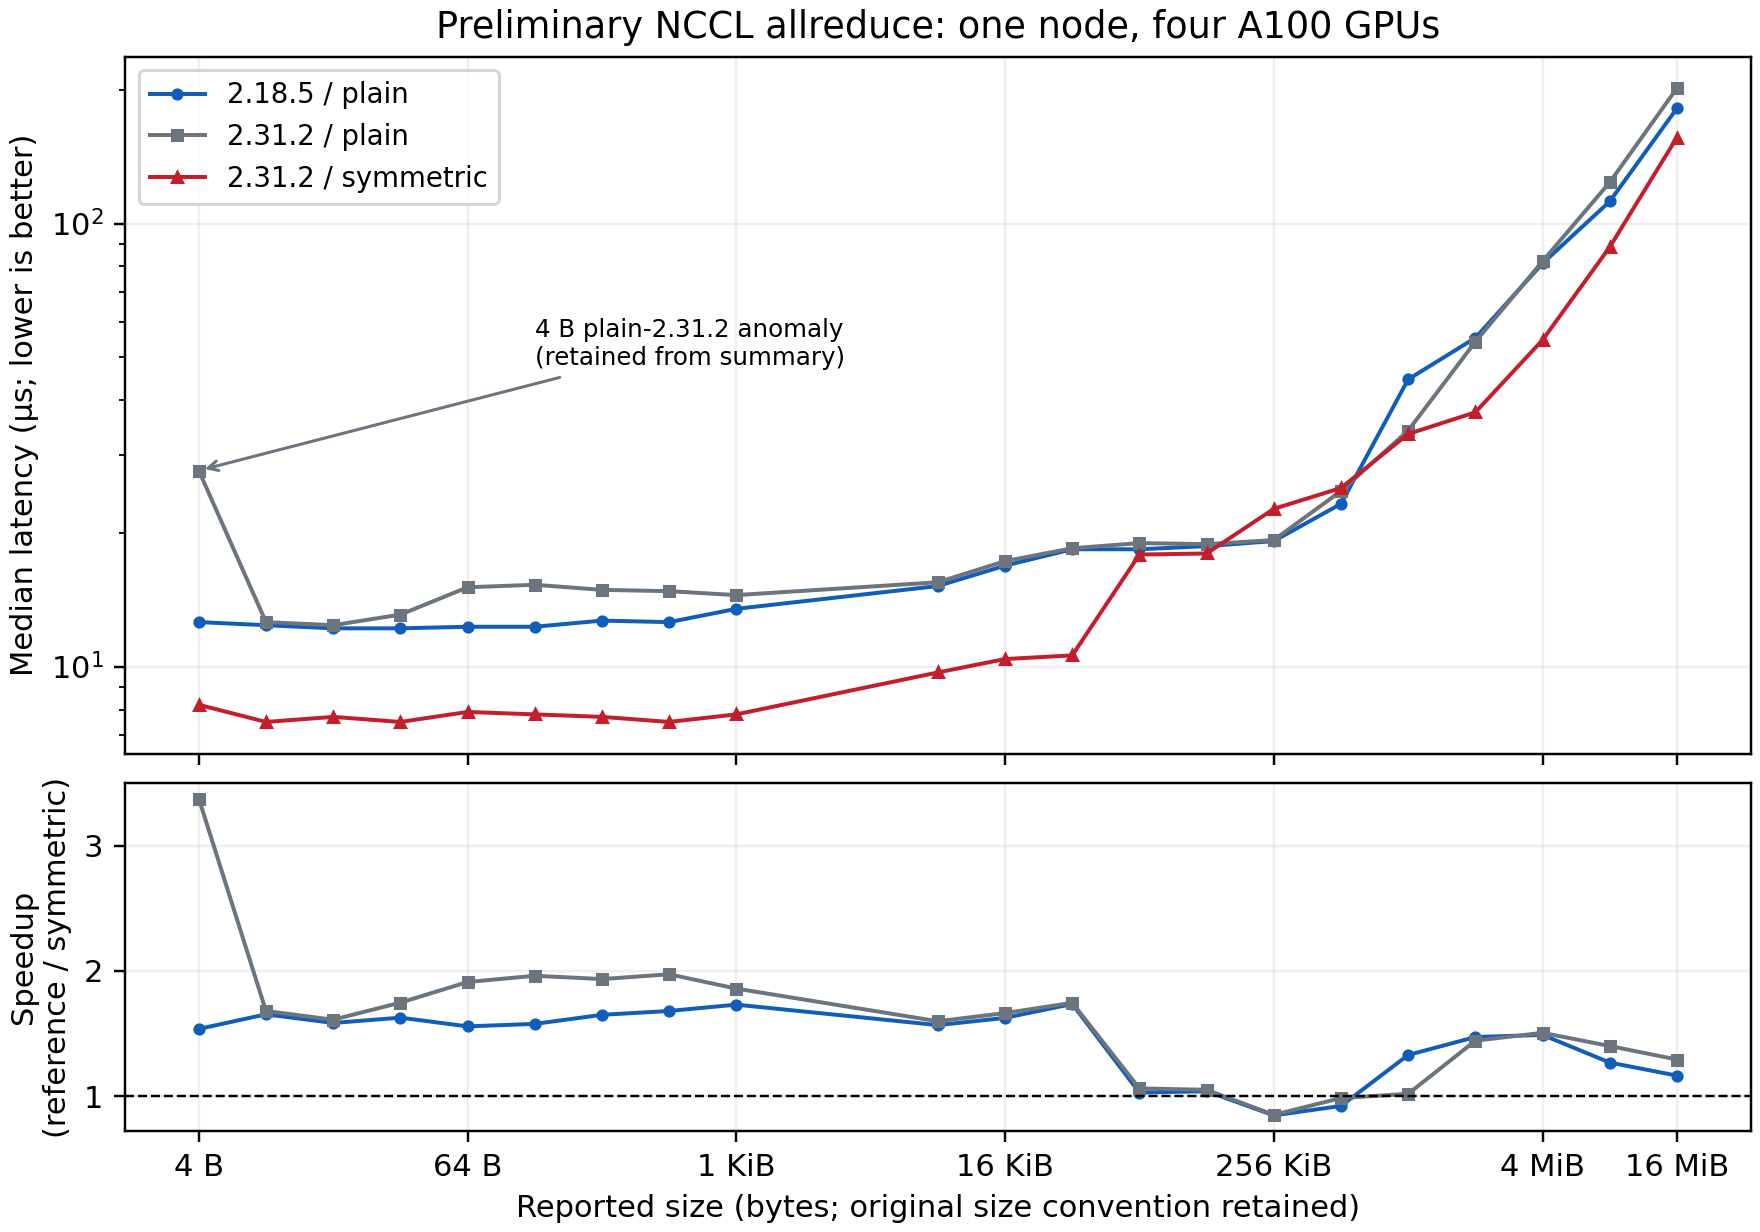
\includegraphics[width=\textwidth]{figures/results/nccl-preliminary-allreduce.png}
\caption{All supplied preliminary allreduce medians. Connecting lines are guides; individual trials and uncertainty intervals are unavailable.}
\label{fig:m-nccl-preliminary-allreduce}
\end{figure}

The eight-byte cell is a candidate for a matched FP64 experiment, not already an estimate of aCG's scalar cost: datatype, invocation mode, and completion boundary remain unresolved.

\subsection{All-to-All Does Not Share the Small-Message Gain}

Small-message all-to-all changes little between the plain and symmetric 2.31.2 configurations, and both are slower than 2.18.5 over the supplied 64\,B--32\,KiB cells. Larger messages show a modest benefit; at 16\,MiB the symmetric configuration is approximately 1.19 times faster than plain 2.31.2.

\begin{figure}[htbp]
\centering
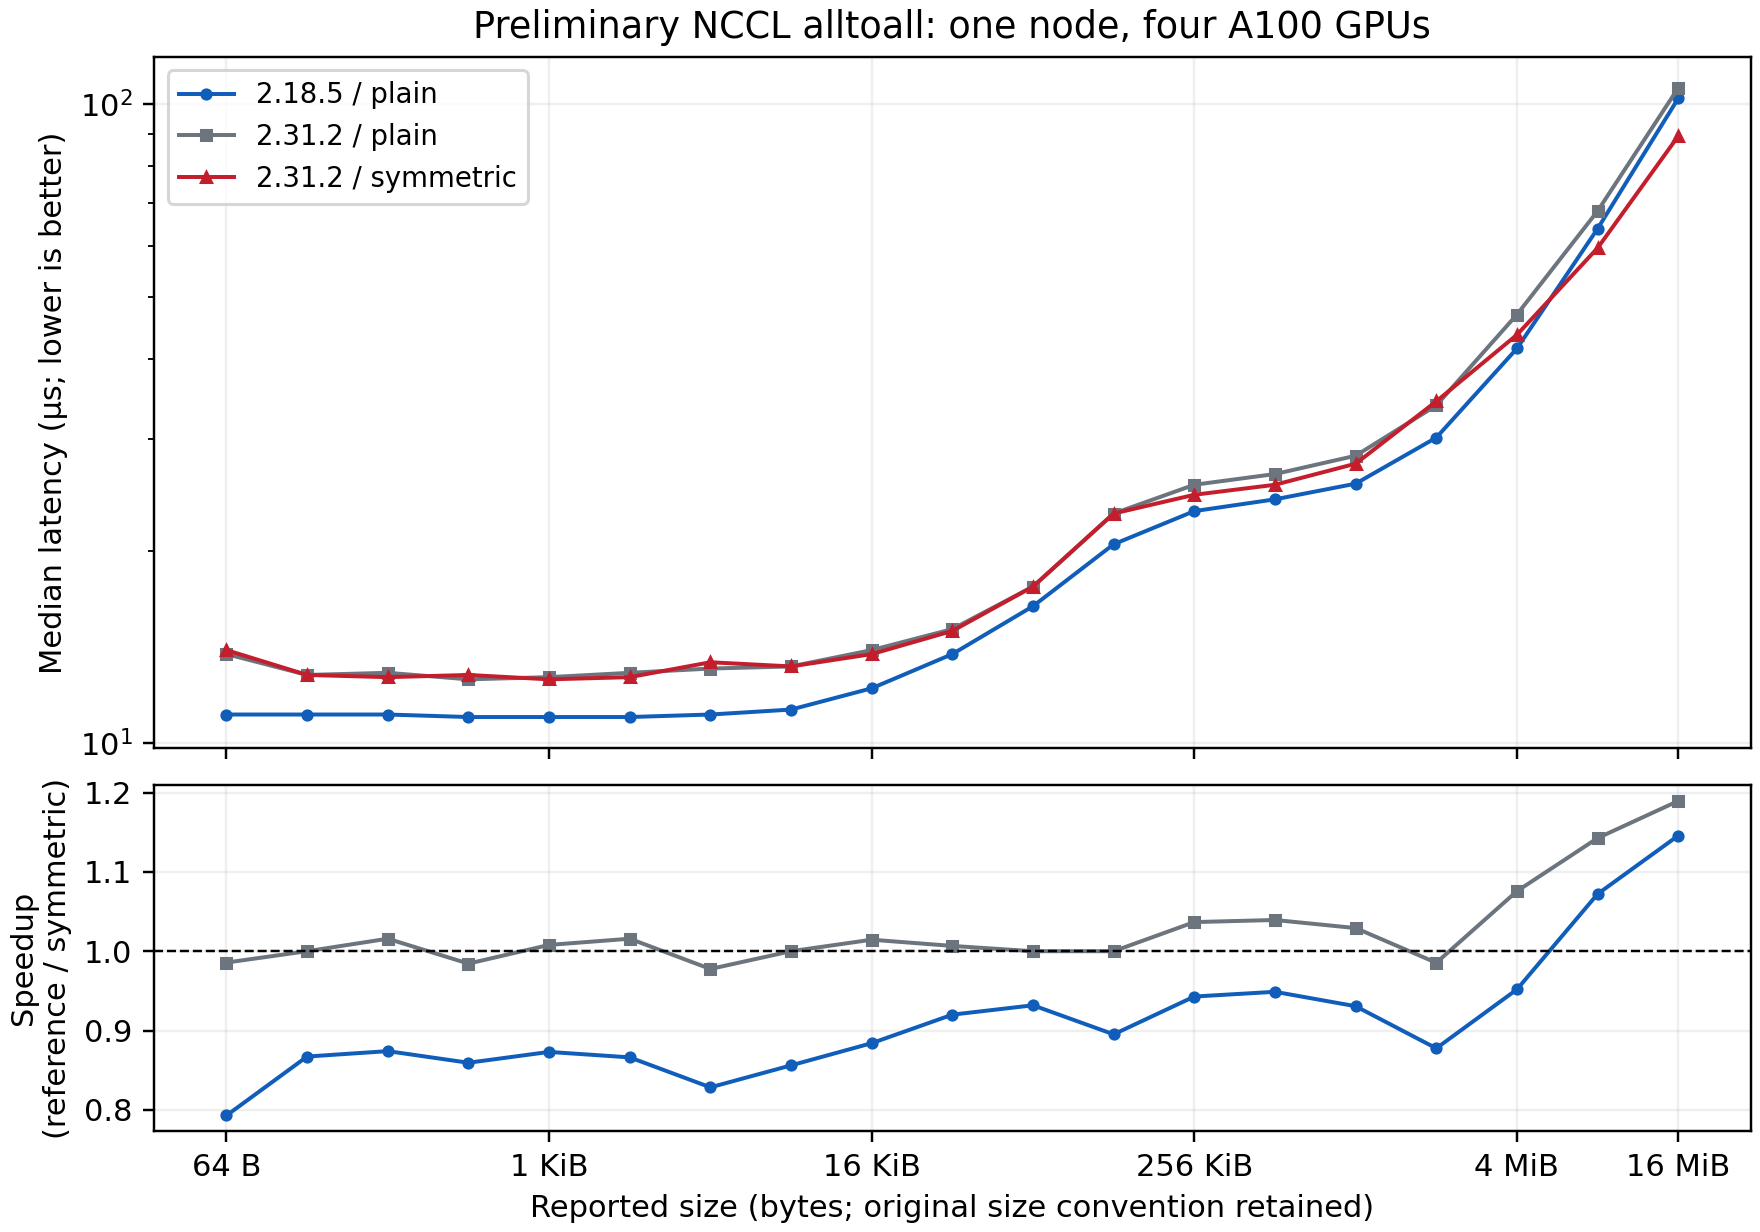
\includegraphics[width=\textwidth]{figures/results/nccl-preliminary-alltoall.png}
\caption{All supplied preliminary all-to-all medians. The size convention is retained from the source summary and is not equated with the main per-peer sweep.}
\label{fig:m-nccl-preliminary-alltoall}
\end{figure}

Source-directory observations alone cannot establish which NCCL kernel produced a timing. Host collectives, grouped point-to-point calls, and user device-API kernels are different paths \cite{nvidia_nccl_collectives_2026,nvidia_nccl_registration_2026}. The reported inter-node proxy regressions and GDAKI stalls lack timing tables and diagnostic logs, so they supply no numerical comparison or established failure cause. The controlled follow-up is a verified one-double intra-node reduction with explicit invocation and completion metadata, followed by an application change only if its benefit persists.
